%%%%%%%%%%%%%%%%%%%%%%%%%%%%%%%%%%%%%%%%%%%%%%%%%%%%%%%%%%%%%%%%%%%%%%

\documentclass[useAMS,usenatbib,a4paper]{mn2e}

\voffset=-0.6in

% Packages:
\input psfig.sty
\usepackage{xspace}
\usepackage{graphicx}
\usepackage{amssymb}
\usepackage{amsmath}

% Macros:
% Making life easier
\newcommand{\be}{\begin{equation}}
\newcommand{\ee}{\end{equation}}
\newcommand{\bs}{\begin{split}}
\newcommand{\bea}{\begin{eqnarray}}
\newcommand{\eea}{\end{eqnarray}}

% Useful symbols
\newcommand{\om}{\Omega_m}
\newcommand{\ha}{\frac{1}{2}}
\newcommand{\ahub}{\frac{\dot{a}}{a}}
\newcommand{\ode}{\Omega_{de}}
\newcommand{\Oe}{\Omega_{e}}
\newcommand{\lcdm}{$\Lambda$CDM}
\newcommand{\neff}{N_{\rm eff}}
\newcommand{\hfid}{H^2_{\rm fid}}
\newcommand{\dl}{\delta}
\newcommand{\sumu}{\Sigma m_\nu}
\newcommand{\mnu}{\Sigma m_\nu}
\newcommand{\mpci}{\,{\rm Mpc}^{-1}}

\newcommand{\dataext}{\data_{\rm ext}}
\newcommand{\transferext}{\mathbf{R}_{\rm ext}}
\newcommand{\smat}{\mathbf{S}}
\newcommand{\cmat}{\mathbf{C}^{\epsilon}}
\newcommand{\cmatext}{\mathbf{C}^{\epsilon_{\rm ext}}}
\newcommand{\noisemat}{\mathbf{N}^{\epsilon}}
\newcommand{\noisematext}{\mathbf{N}^{\epsilon_{\rm ext}}}
\newcommand{\noisematinv}{\left(\noisemat\right)^{-1}}
\newcommand{\noisemattransfer}{\tilde{\mathbf{N}}^{\epsilon}}
\newcommand{\noisemattransferext}{\tilde{\mathbf{N}}^{\epsilon_{\rm ext}}}
\newcommand{\noisemattransferinv}{\left(\tilde{\mathbf{N}}^{\epsilon}\right)^{-1}}
\newcommand{\noisemattransferextinv}{\left(\tilde{\mathbf{N}}^{\epsilon_{\rm ext}}\right)^{-1}}

% Macros
\newcommand{\half}{\frac{1}{2}}
\newcommand{\rhocrit}{\rho_{\rm crit}}
\newcommand{\rvir}{r_{\rm vir}}
\newcommand{\mvir}{m_{\rm vir}}
\newcommand{\kv}{\mathbf{k}}
\newcommand{\xv}{\mathbf{x}}
\newcommand{\mv}{\mathbf{m}}
\newcommand{\muv}{\bm \mu}
\newcommand{\hmsun}{h^{-1}M_{\odot}}
\newcommand{\hmpc}{h^{-1}Mpc}
\newcommand{\hgpc}{h^{-1}{\rm Gpc}}

%%% "Data" - i.e., the observed CMB temperature map
\newcommand{\data}{\mathbf{d}}
%%% Parameters: gravitational potential
\newcommand{\Pot}{\Phi}
\newcommand{\Potvector}{\boldsymbol{\Pot}}
%%% "Signal" - i.e., zero-noise CMB temperature
\newcommand{\signal}{\mathbf{s}}
%%% "noise" - i.e., the pixel noise realization
\newcommand{\noise}{\mathbf{n}}
%%% Transfer function relating the 3D gravitational potential to the
%%% 2D CMB temperature (or other) map
\newcommand{\transfer}{\mathsf{R}}
%%% Signal and noise covariance matrices
\newcommand{\Smat}{\mathsf{S}}
\newcommand{\Nmat}{\mathsf{N}}
\newcommand{\Psimat}{\mathsf{\Psi}}
\newcommand{\Sigmamat}{\mathsf{\Sigma}}
\newcommand{\Cmat}{\mathsf{C}}
%%% Gravitational potential represented as a vector of "voxels" or similar
\newcommand{\gravpot}{\bm \Psi}
%%% Normal (Gaussian) distribution
\newcommand{\normdist}{\mathcal{N}}
%%% Probability theory
\newcommand{\pr}{{\rm Pr}}


%%%%%%%%%%%%%%%%%%%%%%%%%%%%%%%%%%%%%%%%%%%%%%%%%%%%%%%%%%%%%%%%%%%%%%

\title[The 3D Potential of the Universe from CMB Data]
{The Music of the Sphere: I. Inferring the 3D Gravitational Potential
of the Universe on the Largest Scale from Cosmic Microwave Background
Observations}
\author[Blandford et al.]{%
    Roger~D.~Blandford,$^{1}$\thanks{\rdbemail}
    Philip~J.~Marshall,$^{1}$
    Laurence Perrault Levasseur$^{1}$
    \medskip\\
    $^1$\kipac
}


%%%%%%%%%%%%%%%%%%%%%%%%%%%%%%%%%%%%%%%%%%%%%%%%%%%%%%%%%%%%%%%%%%%%%%

\begin{document}

\date{to be submitted to arxiv}
\pagerange{\pageref{firstpage}--\pageref{lastpage}}\pubyear{2015}

\maketitle

\label{firstpage}
%%%%%%%%%%%%%%%%%%%%%%%%%%%%%%%%%%%%%%%%%%%%%%%%%%%%%%%%%%%%%%%%%%%%%%
\begin{abstract}
A method is described that uses observed temperature fluctuations in
the Cosmic Microwave Background to infer the three dimensional
gravitational potential of the universe on the largest scale. It is
demonstrated that the inferred gravitational potential defined on the
last scattering surface can be combined with a prior of almost
scale-free primordial fluctuations (as reported) to infer the
Newtonian potential interior to this surface on our past lightcone as
well as a modest distance beyond our current horizon. This method is
demonstrated and refined using  trial data sets and some limitations
of the approach are uncovered. The refined method is then applied to
the most recent Planck data set and a likelihood analysis used to
define low harmonic Fourier coefficients for the potential with
uncertainties with comoving linear resolution $\sim5$~Gpc. This
approach can be extended and improved to include microwave background
polarization and lensing observations, ``local'' information from
photometric and spectroscopic galaxy and quasar surveys and upcoming
studies of the epoch of reionization. It can also be used to
characterize the particular physical conditions of our universe during
the epoch of inflation and to furnish novel tests of the Gaussianity
hypothesis.
\end{abstract}
% Full list of options at http://www.journals.uchicago.edu/ApJ/instruct.key.html
\begin{keywords}
  cosmology
\end{keywords}
\setcounter{footnote}{1}
%%%%%%%%%%%%%%%%%%%%%%%%%%%%%%%%%%%%%%%%%%%%%%%%%%%%%%%%%%%%%%%%%%%%%%

\section{Introduction}

The earliest astronomical investigations concerned the motion of the
nearby sun, moon and planets  and the positions of the ``fixed'' stars
projected onto the celestial sphere and organized into constellations.
When combined with understanding of the inverse square laws of light
and gravity, this ultimately led to a physics-based, 3D description of
the Milky Way Galaxy. The situation today with the study of the
universe is somewhat analogous. We have extensive surveys of the
locations and motions of nearby galaxies, and their constituents, plus
a detailed Cosmic Microwave Background (CMB) map of the surface of a
sphere with comoving radius $13.9$~Gpc. The general theory of
relativity has been affirmed in many ways and we have an empirical
description of the primordial fluctuations that grew into contemporary
large scale structure and which is consistent with the expectation of
the simplest version of inflation. This has led to a standard
cosmological model of a spatially flat, evolving universe containing
baryonic and dark matter, photons and neutrinos together with a
cosmological constant. This comparatively simple description is
broadly consistent with all current observations but is still not well
enough tested to be accepted as proven. In particular, the
acceleration of the universe might be driven by a more complex dark
energy field and we still lack identification of dark matter and
understanding of the physics underlying inflation. However, the
traditional aspiration of astronomers, to describe the world around
them, has been largely displaced by statistical investigations
designed to elucidate the underlying physics, a program that has made
great progress and which still carries great promise.

In this paper, we seek to initiate a new approach to creating a 3D map
of our universe an activity which, we believe has been relatively
neglected. To use a time series metaphor, we we want to listen to the
music as well as know that it can be represented as a ``flicker''
power spectrum. Most mapping attention, to date, has gone into a
``bottom up'' strategy -- exploring the local group, nearby rich
clusters and the local supercluster along with distinct features such
as the ``Great Attractor'' and the ``Bo\"otes Void''. Large catalogs
of galaxies and clusters have been created with great effort but these
are, now, largely seen as a means to a physics end. Our approach, by
contrast, will be ``top down'' and we shall begin in this paper by
asking the question ``What can we learn about the structure of the
universe on the largest scale from CMB observations from temperature
fluctuations alone?''. We shall show that the high accuracy of the low
$\ell$ Planck observations implies values for the underlying Fourier
expansion coefficients for the Newtonian potential which can be
assembled to produce a 3D density and velocity map with linear
resolution of $\sim3$~comoving Gpc. We shall suggest that it is not
the accuracy of raw measurements themselves that is limiting the
accuracy of this map but uncertainty in our understanding of the
Galactic foreground an error that should diminish with time as a
corollary of the effort to understand polarization maps on finer
angular scale. By contrast, the current uncertainty in the underlying
cosmological model is relatively unimportant we shall adopt the
standard model uncritically.

While we argue that mapping our universe on the largest scale has
intrinsic interest and popular appeal, we also point out that it is
can be a serious contributor to acquiring a deeper understanding of
the fundamental principles that govern its origin and evolution. For
example, knowing whether a particular region of a large survey is
over- or under-dense relative to the cosmic average can supply an
important prior to a measurement of the Hubble constant or the
equation of state of dark matter. Even more enticing is the prospect
of not only projecting the observed state of the universe at
recombination forward in time but backwards, even as far as the
putative epoch of inflation when the structure that has only recently
entered our horizon last left it. Polarization observations turn out
to be particularly valuable for this exercise. In all of these
investigations, we focus on the character of the particular universe
we inhabit as opposed to the nature of the ensemble from which it is
conjectured to have been selected (by us) within the multiverse.
Interestingly, this specificity can extend, some small way into a
statistical fog beyond our current horizon to reveal structure that
will be revealed to our descendants tens of Gyr in the future.
Describing the very largest scale structure that is in some way
knowable raises some important questions of definition and principle
that we shall attempt to clarify.

An essential ingredient of this technique is the assumption that the
largest scale Fourier components describing the initial fluctuation
spectrum are statistically independent and drawn from a Gaussian
distribution with variance that scales with wavenumber according to a
power law inferred on the basis of observations throughout the entire
CMB angular spectrum. Its use for the present purpose is, in some
sense, an extrapolation as its form could not be inferred from the
relatively few modes that we employ here. Addition tests of
``gaussianity'' are therefore quite important to validate our
approach. It is possible to devise nonparametric tests of the
statistical independence of the Fourier modes by considering the
nesting of the equipotential surfaces inferred on both the sphere of
last scattering and the continuation into the interior of this sphere.
The nesting can be described using an equivalent tree.

The results reported in this paper are seen as only the first step in
the full program and only provide a proof principle using the lowest
$\ell$ modes. More sophisticated methods are needed to improve the
linear resolution of the map using higher $\ell$ CMB modes as well as
line of sight investigations of gravitational lensing and the
Integrated Sachs-Wolfe effect. In addition, the accuracy of the map
can be greatly improved by adding measurements made locally using
galaxy, radio source and quasar surveys both completed and proposed.
In addition, if it is possible to make all sky measurements of
$\lambda21$~cm lines from the Epoch of Reionization (EoR) this will
help tie down the large scale potential variation at comoving radii
$\sim10$~Gpc. The methods that will be needed to combine essentially
homogeneous CMB data with quite heterogeneous survey and EoR data are
quite varied and idiosyncratic but should eventually improve the
accuracy and resolution of the maps considerably.

In Sec.~2 of this paper, we will define the gravitational potential
$\Phi$ and explain why it is the best quantity to use for mapping the
universe. We will also show how to evolve it on our past lightcone so
that its value today amounts to measuring it back to the epoch of
inflation so long as we adopt the standard cosmological model. In
Sec.~3, we explain the Gaussian prior on the initial potential
fluctuation spectrum and outline a simple, Bayesian procedure to infer
the Fourier modes needed to make the 3D map. We also outline a
procedure to quantify the error in the derived map. This is followed
in Sec.4 with a description of the tests that we have carried out
using trial datasets to optimize and validate our this procedure and a
brief discussion of how it will have to be modified to accommodate
additional input data. The main result of this paper is the very low
resolution map of the universe based on Planck temperature fluctuation
data alone and this is presented and discussed in Sec.~5. In Sec.~6,
we summarize our main conclusions and preview the topics we shall
discuss in Paper II (polarization and inflation), Paper III
(non-parametric tests of gaussianity) and Paper IV (inclusion of
additional datasets).

%%%%%%%%%%%%%%%%%%%%%%%%%%%%%%%%%%%%%%%%%%%%%%%%%%%%%%%%%%%%%%%%%%%%%%

\section{The Potential of the Universe}

\subsection{Potential vs Density Mapping}

We begin by clarifying some simple choices. The map of the universe
that we will make is one of the linearized Newtonian potential
perturbation $\Phi$ from a spatially homogeneous world model. (We set
$c=1$.) This is equivalent to (minus half) the perturbation to the
$g_{00}$ component of the metric in the Newtonian gauge and also to
the (scaled) curvature perturbation on the scales that we are
considering. (Tensor perturbations require additional metric
perturbations but are demonstrably small enough to ignore.) Our
reasons for choosing potential over density are that it does not
change until it re-enters the horizon and then is constant through the
Einstein-De Sitter phase before decreasing by 22 percent on all
relevant scales after the cosmological constant becomes important. Our
time coordinate will be the same as the cosmological time $t$ that is
used to describe the corresponding homogeneous cosmology. (Alternative
time coordinates are useful in the early universe, a topic to which we
return in Paper 2.) We adopt comoving spatial coordinates, $\bf x$, in
the background universe, using the local, CMB rest frame to fix the
origin.

\subsection{Standard Cosmology and Potential Evolution}

We adopt a Flat $\Lambda$CDM cosmology with Planck parameters
($\Omega_\Lambda=0.69$, $H_0=68$~km s$^{-1}$ Mpc$^{-1}$) and evolve
both the background cosmology and the linear potential perturbations
according to standard equations from the time. Our results are quite
insensitive to this choice within the range spanned by alternative
measurements, as we affirm below. The comoving radius of the big bang
is $x=14.2$~Gpc and of recombination $x=13.9$~Gpc. Other important
epochs are identified in Fig.~1a. We set the comoving radius of
recombination henceforth as our unit of length.

We use the solutions of the standard cosmological perturbation
equations to relate the potential at recombination to its value today
which is what we will ultimately exhibit. We show this evolution in
Fig.1b.
\begin{figure}[t]
\centering
%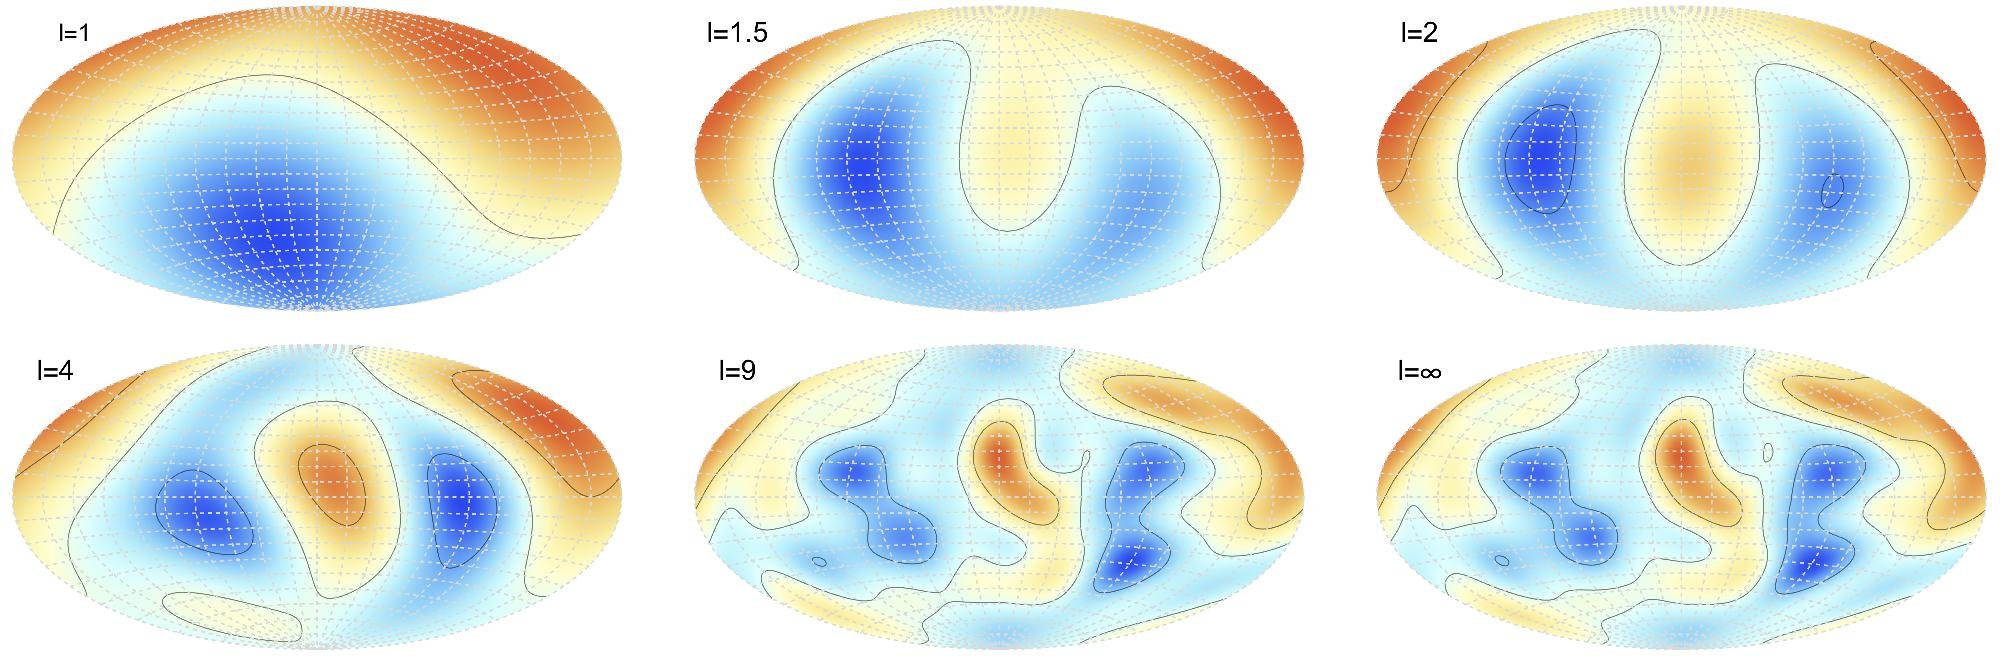
\includegraphics[width=4in]{figures/fig1.pdf}
\caption{\small{a) The local universe interior to the CMB photosphere expressed in comoving coordinates. The circles are, in order, $a=0.6$, ($z\sim0.7$), schematically the limit of present surveys, $a=0.3$, ($z\sim2$) roughly the effective limit of future surveys, the nominal Epoch of Reionization at $a=0.1$, ($z\sim9$ and the CMB photosphere at $a=0.00093$, ($z\sim1100$) and a distance $x=1$. The comoving radius of the big bang is $14.2$~Gpc. Also shown as dashed lines are the nodes of a single wave mode with $k\sim0.45$~Gpc$^{-1}$ which contributes significantly to spherical harmonics with $\ell\leq8$. b) Variation of the amplitude of this wave with scale factor $a$.}}
\end{figure}

\subsection{Fourier Expansion of the Potential}

It is conventional to Fourier expand the potential $\Phi({\bf x}$
today. Although the full spectrum of the Fourier modes we are
discussing is continuous in ${\bf k}$ (where $\bf k$ is measure in
units of (13.9~Gpc)$^{-1}$, the fact that our observations are made
over a restricted volume means that we can treat the waves as a
discrete Fourier transform of modes associated with a box in comoving
space of side $L$ on which periodic boundary conditions are imposed.
If $L$ is too small, the enforced periodic boundary conditions will
strongly distort the map; if $L$ is too large, the mode spacing in
k-space will be too fine and the modes will not be independent. $L$ is
chosen here to have a compromise value of $L=4$, which we discuss
further below.
\begin{equation}
\Phi[{\bf x}(r,\theta,\phi)]=\sum_{n=1}^{N/2}[f_n\cos({\bf k}_n\cdot{\bf x})+f_{N+1-n}\sin({\bf k}_n\cdot{\bf x})]
\end{equation}
where the coefficients $f_n$ are real and ${\bf k}=\Delta k{\bf
n}=\Delta
k\{n_1,n_2,n_3\}=k\{\sin\theta'\cos\phi',\sin\theta'\sin\phi',\cos\theta'\}$,
with $n_1,n_2,n_3$ integers and $\Delta k=2\pi/L=\pi/2$.  We restrict
the sum to $(n_1^2+n_2^2+n_3^2)^{1/2}\le n_{\rm max}$ and only need
consider $\bf k$ over a hemisphere (since the potential must
everywhere be real.) We label the coefficients by the index $n$
running from $1$ to $N\sim4\pi n_{\rm max}^3/3$.
($N=6,32,122,256,514,924,1418,2108,3070,4168$ for $n_{\rm max}=1$
through $10$ which will suffice for this paper.)

\subsection{Sachs-Wolfe Limit}

Our input data comprises CMB temperature fluctuations from
recombination $\delta(\theta,\phi)\equiv\delta T/T$, where
$\theta,\phi$ are spherical polar coordinates measured with respect
the same axes as the $\theta',\phi'$ used for $\bf k$. As we are
confining attention to long wavelength Fourier components we will only
need small $\ell$ spherical harmonics to describe $\delta$. The
transverse scales are large compared with the thickness of the
photosphere and this implies that the dominant cause of the
temperature fluctuation is the gravitational redshift --- the
Sachs-Wolfe effect --- that $\Phi=3\delta$, allowing for the expansion
in the usual manner. This is increasingly inaccurate for
$\ell\gtrsim30$ and we use the more accurate relation between $\delta$
and $\Phi$, though, for this paper the difference is insignificant.

\subsection{Spherical Harmonic Expansion and Response Matrix}

$\delta$ and, consequently, $\Phi({\bf x})$ can be expanded formally
as a finite sum of spherical harmonics --- the generalisation of
Fourier modes to a sphere --- up to and including the $\ell_{\rm max}$
shell:
\begin{equation}
\Phi=\sum_1^{(\ell_{\rm max}+1)^2}a_yY_y
\end{equation}
where $Y_y$ is a vector of real spherical harmonics:
\begin{equation}
Y_y(\theta,\phi)=\{Y_{0,0},Y_{1,0},2^{1/2}\Re[Y_{1,1}],2^{1/2}\Im[Y_{1,1}],Y_{2,0},\dots,2^{1/2}\Im[Y_{\ell_{\rm max},\ell_{\rm max}}]\}
\end{equation}
of length $(\ell_{\rm max}+1)^2$ and where $\theta,\phi$ are standard spherical polar coordinates. Note that there are $2\ell+1$ independent, real, basis function in each $\ell$-shell. (The use of a real basis helps identify systematic effects.) Note also that $\int d\Omega Y_yY_{y'}=\delta_{yy'}$. It is convenient to treat $\ell_{\rm max}$ as a continuous variable by adding a fraction between zero and unity of the largest $\ell$ shell and thereby change the angular resolution continuously.
\begin{figure}[t]
\centering
%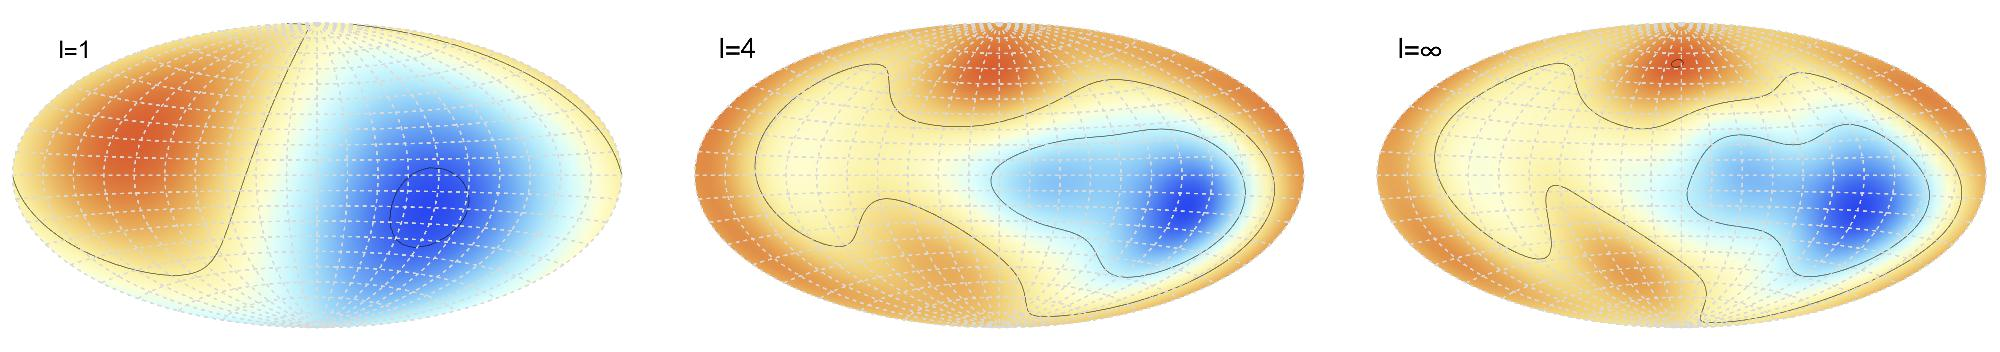
\includegraphics[width=6in]{figures/fig2.jpg}
\caption{{\small Photospheric potential fluctuations of the CMB for $\ell_{\rm max}=2,4.5,10$ (derived from Planck data) and shown as Mollweide projections.}}
\end{figure}

We wish to relate a specific realization of the CMB temperature
fluctuations to the underlying Fourier  spectrum. We first expand
$\Phi({\bf x})$ as a finite sum of Legendre polynomials:
\begin{equation}
\Phi({\bf x;\ell_{\rm max}})=\sum_{\ell=0} ^{\ell_{\rm max}}(2\ell+1)\sum_{n=1}^{N/2}j_{\ell}(k_nx)P_{\ell}({\hat{\bf k}}_n\cdot{\hat{\bf x}})[\cos(\ell\pi/2)f_n+\sin(\ell\pi/2)f_{N+1-n}].
\label{eqphisum}
\end{equation}
We next introduce the response matrix ${\mathbf R}_{yn}$ which relates
individual Fourier coefficients to spherical harmonic coefficients on
the recombination sphere $x=1$.
\begin{equation}
a_y={\mathbf R}_{yn}f_n.
\end{equation}
Using Eq.~(\ref{eqphisum}), we find that
\begin{equation}
\mathbf{R}_{yn}=4\pi Y_y(\theta'\phi')j_\ell(k)[\cos(\pi\ell/2),\sin(\pi\ell/2)]\ {\rm for}\ [1\le n\le N/2,\ N/2<n\le N].
\end{equation}
Typically, the length of $f_n$ will exceed that of $a_y$ and we must
find the most likely values of $f_n$ for a given vector $a_y$.

\subsection{Monopole and Dipole Components}

The sums over $y$ include the monopole and dipole terms. These are in
a sense unknowable because we do not know the CMB temperature at this
time averaged over a volume larger than our horizon and we cannot
remove the peculiar motion of the Earth sufficiently carefully to
measure the $\ell=1$ coefficients. However, Planck does report these
values\dots


%%%%%%%%%%%%%%%%%%%%%%%%%%%%%%%%%%%%%%%%%%%%%%%%%%%%%%%%%%%%%%%%%%%%%%

\section{Reconstruction of the Interior Potential}

\subsection{Gaussian Prior}

The ``holographic'' reconstruction that we are attempting has a
fundamental limitation in that $O(\ell_{\rm max}^3)$ Fourier
components $f_n$ are needed fro $O(\ell_{\rm max}^2)$ spherical
harmonic coefficients $a_y$. We need additional constraints. One
source of these, important for low resolution reconstruction, comes
for highly accurate temperature measurements which imply, in practice,
that high order $a_y$ can contribute to low order $f_n$. That this is
not sufficient can be seen by considering the problem of inferring the
interior temperature of the Earth from very accurate surface
measurements alone. We would have no way of distinguishing a solution
where the isotherms extended into the core, well spaced from the
correct answer where they are bunched up just below the surface. In
the present case, the additional information is contained in our
hypothesis that the $f_n$ are drawn from a Gaussian distribution with
variance satisfying:
\begin{equation}
\sigma_\mathbf{n}^2=\sigma_1^2n^{n_s-4},
\end{equation}
where $n_s$ is measured to be 0.96 (1 suffices for the present
purpose) and $\sigma_1^2/2\pi^2L^3\equiv\frac{d<\Phi^2>}{d\ln k}$, the
dimensionless variance of a mode with $k=\Delta k$ today is measured
to be ???. We reiterate that the spectrum of the power law is derived
from a study of the full range of spherical harmonics,
$2\le\ell\lesssim5000$ not just from the modes that are actually used
in the analysis. We discuss the sensitivity of our maps to the chosen
spectrum and the assumption of Gaussianity below.

\subsection{Maximum Likelihood Estimator}

We now explain how to characterize the posterior PDF (which under our
assumptions is a multi-variate Gaussian distribution) for each of the
coefficients $f_n$ by first finding its peak, minimizing the quantity
\begin{equation}
-2\ln{\cal P}\left(f_n|a_y\right) \approx (a_y- f_n\mathbf{R}_{ny})C_{yy'}^{-1}(a_{y'}-\mathbf{R}_{y'n'}f_{n'})+\frac{f_n^2}{\sigma_{{\bf n}}^2} + \mathrm{const.}
\end{equation}
with respect to variation of $f_n$. Here, $C_{yy'}^{-1}$ is the
inverse of the covariance matrix. This leads to the linear equations:
\begin{equation}
f_n=\left(\mathbf{R}_{ny}C_{yy'}^{-1}\mathbf{R}_{y'n'}+\frac{\delta_{nn'}}{\sigma_{\bf n}^2}\right)^{-1}\mathbf{R}_{n'y}C_{yy'}^{-1}a_{y'}
\label{eq:bayes}
\end{equation}

\subsection{Uncertainties}

This is an approach that should produce values for the $f_n$ as long
the covariance matrix is well-defined. This does not guarantee that
they are meaningful and in order to do this, we must devise a
procedure to estimate their significance.

%%%%%%%%%%%%%%%%%%%%%%%%%%%%%%%%%%%%%%%%%%%%%%%%%%%%%%%%%%%%%%%%%%%%%%

\section{Testing the Method}

\subsection{Recovering a Trial Potential}

Before applying this method to the Planck dataset, we should
investigate its performance with trial data. We have created 100 mock
datasets with $L=4$, $n_\mathrm{max}=4$ and used these to answer some
of the questions we have already raised. For each mock dataset, we
assign {\it true} Fourier coefficients $f_\mathrm{n\,true}$ adopting
the Gaussian prior and using a random number generator. We next
convert these to {\it measured} $f_n$ using the Planck covariance
matrix. We then create a CMB map on the recombination sphere and
evaluate the spherical harmonic coefficients $a_y$ up to
$\ell_\mathrm{max}=8$. The final step is to use our procedure to
recover {\it derived} coefficients $f_\mathrm{n\,der}$ which can be
compared with the true values. We adopt a crude  figure of merit for
each mock map:
\begin{equation}
F=\frac1N\sum_{n=1}^N\left(\frac{f_\mathrm{n\,der}-f_\mathrm{n\,true}}{\sigma_{\mathbf n}}\right)^2.
\end{equation}
In Fig.~ we compare examples of derived maps with different figures of
merit with the original true map. We adopt a figure of merit $F=???$
as an acceptable value for a map.

\subsection{Box Size}

As a first step towards optimizing this procedure, we consider the
size of the box, $L$. We repeat the process we have just described for
larger and smaller values of $L$ to confirm that we have chosen the
best value.

\subsection{Sensitivity to the Cosmological Model}

We can also confirm that our answers are not sensitive to the assumed
cosmological model. We have separately changed $\Omega_\Lambda$ and
$\Omega_k$ each by  0.05 and we have also consider dark energy models
with $w=-0.9$. We find that $F$ hardly changes.

\subsection{Variation with $n_\mathrm{max}$}

We next consider how the figure of merit is improved as we increase
the number of Fourier components, i.e. by increasing $n_\mathrm{max}$.
The maximum value that can be used clearly depends upon the accuracy
of the measurement of individual Fourier components. We find that with
the covariance matrix we have adopted, which is based upon the
properties of the Planck data, there is no significant improvement in
the figure of merit by increasing $n_\mathrm{max}$.Furthermore, if we
reduce the variance by as much as a factor 3, we find only a marginal
reduction in $F$ when $n_\mathrm{max}$ is increased by one. However,
if we increase $\ell_\mathrm{max}$ from 8 to 12 we find that we can
improve the accuracy and increase the resolution of the map by
increasing $n_\mathrm{max}$ from 10 to 12. We will discuss how to do
this with the existing data by using a more complicated estimator in
Paper IV.

%%%%%%%%%%%%%%%%%%%%%%%%%%%%%%%%%%%%%%%%%%%%%%%%%%%%%%%%%%%%%%%%%%%%%%

\section{Application to the Planck Data Set}

\subsection{Description of Dataset}

In our first attempt to create 3D map we take $N_m=100$ individual
Planck sky maps and sample them using the HEALPIX algorithm and then
create $N_m$ sets of spherical harmonic coefficients which we convert
to out basis to derive $N_m$ sets of coefficients $a_y$. We then used
this to recreate the mean coefficients $\bar{a}_y$ and the low
resolution sky map. We then constructed a covariance matrix for the
measurements of $a_y$:
\begin{equation}
C_{yy'}=<(a_y-\bar{a}_y)(a_{y'}-\bar{a}_{y'})>
\end{equation}
where the average is over all the $N_m$ individual maps. All we are
doing here is finding linear combinations of the data that are
statistically independent. We find that this matrix is robustly
invertible for $\ell_\mathrm{max}\le8$ and confine our attention to
this straightforward case. be used directly up to $\ell=8$. We
construct the eigenvalues and eigenfunctions of the covariance matrix
both over all values of $\ell$ and separately with $\ell$ shells. We
observe no unusual patterns in these quantities. We were able to
improve the stability of the inversion by renormalizing the
coefficients within $\ell$ shells but will not pursue this and other
strategies here.

\subsection{Derived Potential Map}

We are now in a position to use Eq.~(\ref{eq:bayes}) to solve for the
Fourier coefficients and exhibit the 3D potential map. We also show
the ``true'' $\ell_\mathrm{max}=8$ map and the ``derived'' map which
has a figure of merit $F=???$.  It can be seen that there there are
xxx potential maxima and xxx potential minima within the recombination
sphere today We appear to be close to a potential maximum. We can use
these maps to create distributions of the current fractional density
perturbation (the local underdensity is $\delta\rho/\rho=-???$. In
addition we can create low resolution velocity maps use the
perturbation equations and find a value ${\mathbf v} =???$ towards ???

\subsection{Velocity and Density Maps}

We can use these maps to create distributions of the current
fractional density perturbation. We appear to be close to a potential
maximum with $\delta\rho/\rho=-???$. In addition we can create low
resolution velocity maps use the perturbation equations and find a
value ${\mathbf v} =???$ towards ???. The errors are derived on the
basis of the simulations discussed above.

\subsection{The Universe Beyond our Horizon}

Interestingly, it is possible to make statements about the universe
beyond our current horizon. This is structure that will become visible
in our future. This might seem surprising but it is really a
consequence of our Gaussian prior. To see this suppose our prior were
that there was a single Fourier mode we could then project as far
beyond our horizon as the accuracy with which we could determine the
amplitude and phase and direction of this mode would allow.

\subsection{Influence of Residual Galactic Foreground}

A major concern relating to this approach is that the large scale
structure in our maps is seriously contaminated by the removal of the
Galactic foreground. It is encouraging that he structure that we find
shows little correlation with major features within the Galaxy but
additional tests are underway to quantify this uncertainty.

%%%%%%%%%%%%%%%%%%%%%%%%%%%%%%%%%%%%%%%%%%%%%%%%%%%%%%%%%%%%%%%%%%%%%%

\section{Discussion}

In this paper, we have developed a simple approach to mapping the 3D
Newtonian potential within  the last scattering surface at the epoch
of recombination. As the perturbations inferred on the scales we are
considering remain quite linear, we can use observations from any part
of spacetime on our past lightcone to infer the entire variation
within our horizon (and slightly beyond) from the time of inflation to
the far future. We have deliberately restricted the input data to CMB
temperature fluctuations with $0\ell\leq\ell\leq8$ where the
covariance matrix is easily computed and have set aside the abundance
of data that could improve the map, or may do so in the future, in
order to optimize the method and elucidate the viability and
limitations of this approach. The results are encouraging but also
bring out how hard it will be to connect detailed maps of small
volumes of the universe, especially in our neighbourhood, to structure
on the largest scale. We intend to discuss these and closely related
matters in the next three papers in this series.

%%%%%%%%%%%%%%%%%%%%%%%%%%%%%%%%%%%%%%%%%%%%%%%%%%%%%%%%%%%%%%%%%%%%%%

\section*{Acknowledgments}

We are especially grateful to Planck team members Ingunn Wehus \&
Hans-Kristian Eriksen for their encouragement and help in furnishing
100 samples of the low resolution Planck temperature data to allow us
to complete this pilot project.

\bibliographystyle{apj}
\bibliography{references}
\end{document}
